\documentclass[12pt, twoside]{article}
\usepackage[francais]{babel}
\usepackage[T1]{fontenc}
\usepackage[latin1]{inputenc}
\usepackage[left=4mm, right=4mm, top=4mm, bottom=4mm]{geometry}
\usepackage{float}
\usepackage{graphicx}
\usepackage{array}
\usepackage{multirow}
\usepackage{amsmath,amssymb,mathrsfs}
\usepackage{textcomp}
\pagestyle{empty}
\usepackage{soul}
\usepackage{eurosym}

\begin{document}  


NOM PRENOM: \ldots\ldots \ldots \ldots \ldots  \ldots \ldots \ldots \ldots 


\begin{center}
{\fbox{$3^{e}2$ \qquad \qquad \textbf{\Large{Devoir surveill� 3}}
\qquad \qquad 12/04/2013}}
\end{center}

\bigskip


\textit{\ul{Remarques}: Chaque r�ponse sera r�dig�e et justifi�e. L'exercice 2
se fait sur la photocopie.}

\bigskip

\ul{\textbf{Exercice 1}}: (\textit{4 points})

\begin{enumerate}
  \item Calculer le PGCD des nombres 165 et 210.
  \item Dans une salle de bain, on veut recouvrir le mur situ� au-dessus de la
  baignoire avec un nombre entier de carreaux de fa�ence de forme carr� dont le
  c�t� est un nombre entier de centim�tres le plus grand possible.
  
  \begin{enumerate}
    \item D�terminer la longueur, en cm, du c�t� d'un carreau, sachant que le
    mur meusre 210 cm de hauteur et 165 cm de largeur.
    \item Combien faudra-t-il alors de carreaux?
    \end{enumerate}
\end{enumerate}

\bigskip

\ul{\textbf{Exercice 2}}: (\textit{6 points})

\enskip

\begin{center}
\begin{tabular}{|c|c|c|c|}

\hline

Enonc� & Sch�ma � main lev�e & Calculs & R�ponse \\

\hline

\quad & \quad & \quad & \quad \\

\quad & \quad & \quad & \quad \\

\begin{minipage}{6cm}


ABC est un triangle rectangle en C avec CB=4 cm et $\widehat{ABC}=50$�.


\end{minipage}
&
\begin{minipage}{4cm}
\quad
\end{minipage}
&
\begin{minipage}{6cm}
\quad
\end{minipage}
&
\begin{minipage}{25mm}
CA $\approx$ \ldots 
\end{minipage}

\\

\quad & \quad & \quad & \quad \\

\quad & \quad & \quad & \quad \\


\hline

\quad & \quad & \quad & \quad \\


\quad & \quad & \quad & \quad \\

\begin{minipage}{6cm}


ABC est un triangle rectangle en C avec AB=7 cm et BC=4 cm.


\end{minipage}
&
\begin{minipage}{4cm}
\quad
\end{minipage}
&
\begin{minipage}{6cm}
\quad
\end{minipage}
&
\begin{minipage}{25mm}
$\widehat{ABC}\approx$ \ldots 
\end{minipage}

\\
\quad & \quad & \quad & \quad \\

\quad & \quad & \quad & \quad \\

\hline

\quad & \quad & \quad & \quad \\

\quad & \quad & \quad & \quad \\

\begin{minipage}{6cm}


ABC est un triangle rectangle en C avec AB=7 cm et $\widehat{ABC}=67$�.


\end{minipage}
&
\begin{minipage}{4cm}
\quad
\end{minipage}
&
\begin{minipage}{6cm}
\quad
\end{minipage}
&
\begin{minipage}{25mm}
AC$\approx$ \ldots 
\end{minipage}

\\

\quad & \quad & \quad & \quad \\

\quad & \quad & \quad & \quad \\

\hline
\end{tabular}

\end{center}

\bigskip

\ul{\textbf{Exercice 3}}: (\textit{6 points})


\enskip

\begin{tabular}{cc}
\begin{minipage}{10cm}
L'unit� est le centim�tre.

\begin{enumerate}
  \item Reproduire la figure ci-contre � la taille r�elle.
  \item Calculer l'arrondi au degr� pr�s de l'angle $\widehat{RTI}$.
  \item Calculer l'arrondi au degr� pr�s de l'angle $\widehat{LAI}$.
\end{enumerate}
\end{minipage}
&
\begin{minipage}{8cm}
\begin{center}
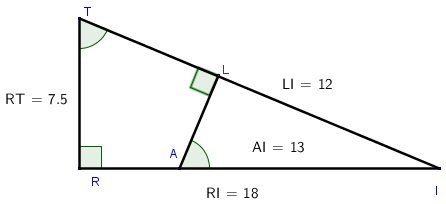
\includegraphics[width=7cm]{images/ex3.jpg}
\end{center}
\end{minipage}
\end{tabular}

\bigskip

\ul{\textbf{Exercice 4}}: (\textit{4 points})


\enskip

\begin{tabular}{cc}
\begin{minipage}{9cm}
Le cercle ci-contre a pour centre O et pour rayon 6 cm.

Calculer l'arrondi de DH � 0,1 cm pr�s.
\end{minipage}
&
\begin{minipage}{9cm}
\begin{center}
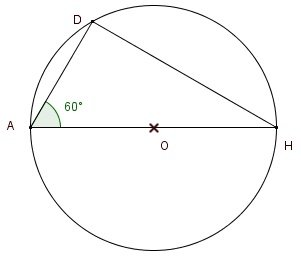
\includegraphics[width=45mm]{images/ex4.jpg}
\end{center}
\end{minipage}
\end{tabular}
\end{document}
